\section{The Experiment Harness}
\label{sec:annex-experiment-harness}

This annex documents the machinery behind Section~\ref{sec:empirical-evaluation}. Its purpose is reproducibility across rounds: a new experiment is a new folder under \texttt{experimentos/}, and the same consolidation, reporting and publishing scripts operate on it unchanged. The harness is deliberately separate from the model code---it only reads what training and deployment write---so an experiment never depends on the library version that produced it, and the library never learns about the campaign that used it.

\subsection{Stages and Records}

Each configuration is one YAML file and one slug. The slug encodes the family and the mixers: \texttt{attn\_nsa\_attn\_\_engram\_attn} is a hybrid pair, \texttt{attn\_single\_mamba} a single-mixer baseline, and the ablations carry their own prefixes (\texttt{opt\_}, \texttt{norm\_}, \texttt{pe\_}, \texttt{trans\_}, \texttt{vit\_}, \texttt{task\_}, \texttt{tokenizer\_}, \texttt{batch\_}, \texttt{realdata\_}, \texttt{audio\_}, \texttt{bitnet\_}). Every run executes the same five stages: train, export the checkpoint, deploy in a standard and a quantized format, evaluate four held-out masked prompts per format, and export the Hugging Face package. A failure in one stage is recorded, does not abort the sweep, and surfaces later as a missing row rather than as a silent zero.

Three recorders write independently and are joined only at reporting time:

\begin{enumerate}[leftmargin=*]
    \item \textbf{The per-step training log.} One CSV per run with one row per optimisation step: loss, accuracy, learning rate, gradient norms per parameter group, clipping ratio, step time and throughput. Round~2 logged 2{,}656{,}372 rows, which are streamed and reduced to per-epoch means before any chart is drawn.
    \item \textbf{The parameter census.} For every configuration, the number of parameters in each module group (attention, embeddings, FFN, head, normalization, positional encoding, mHC, router, residual). This is what separates ``the model is bigger'' from ``the attention block is bigger''.
    \item \textbf{The pipeline ledger.} One row per stage execution with category, status, duration and return code. It is the only record of the failures, and therefore the only source for the reliability analysis.
\end{enumerate}

\begin{figure}[tbp]
\centering
\fitfigure{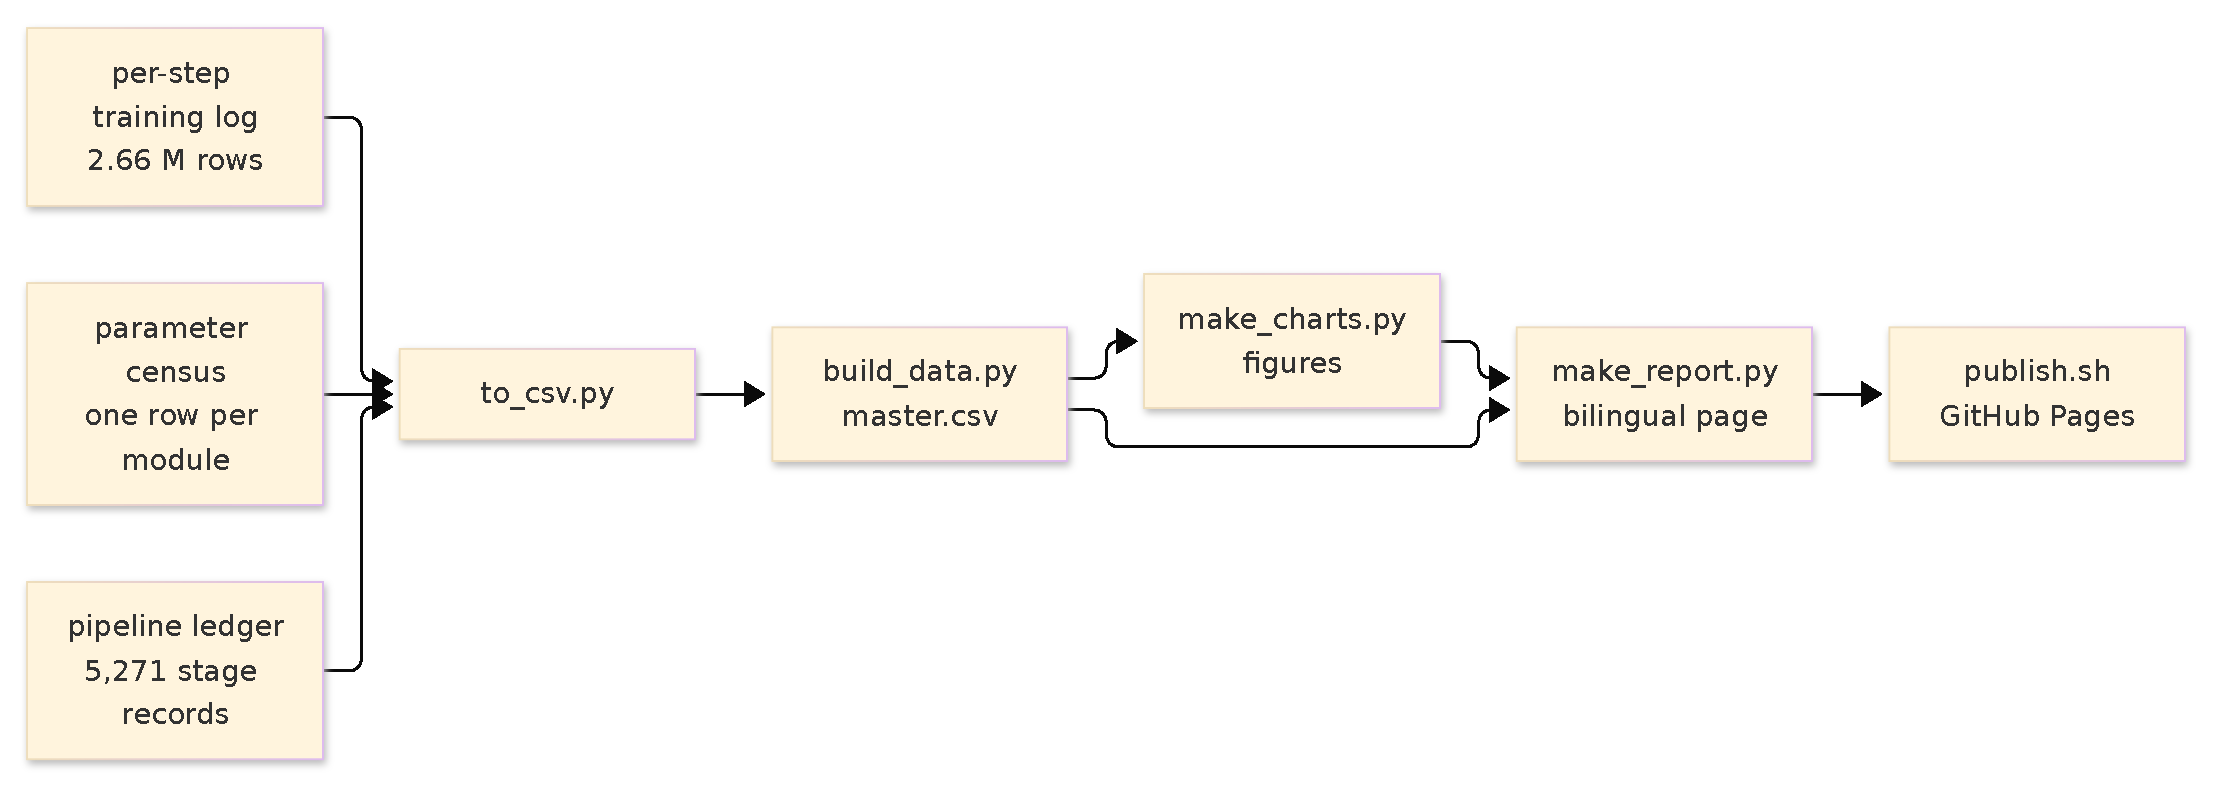
\includegraphics{figures/experiment-reporting.pdf}}
\caption{The offline reporting toolchain. The three recorders are consolidated into CSV files, joined by configuration into \texttt{master.csv}, charted in both themes, and rendered into a bilingual static page with the joined datasets published next to it. Nothing in this chain needs a GPU.}
\label{fig:experiment-reporting}
\end{figure}

\subsection{The Stage Ledger of Round~2}

Table~\ref{tab:stage-ledger} reproduces the ledger. Training dominates both the record count and the cost: 1{,}039 attempts, 868 successes and 171 failures, a median of 68 minutes and a P90 of 84 minutes per successful run, for 906 GPU-hours in total. Deployment is the only other stage that fails (104 times out of 1{,}734), and the failures are symmetric: a configuration whose standard export fails also fails its quantized export, which points to checkpoint or configuration serialisation rather than to quantization. Evaluation and Hugging Face export never failed in the analysed population.

\begin{table}[H]
\centering
\small
\caption{Pipeline stage ledger for Round~2. Durations are seconds; totals are hours of wall-clock across the whole campaign.}
\label{tab:stage-ledger}
\begin{tabular}{lrrrrrr}
\toprule
Stage & Records & OK & Failed & Median (s) & P90 (s) & Total (h) \\
\midrule
Training              & 1{,}039 & 868  & 171 & 4{,}101.45 & 5{,}037.3 & 906.0 \\
HF export             & 867     & 867  & 0   & 17.41      & 44.7      & 5.4   \\
Inference evaluation  & 1{,}630 & 1{,}630 & 0 & 10.37      & 13.1      & 4.9   \\
Deployment            & 1{,}734 & 1{,}630 & 104 & 8.64     & 38.0      & 8.8   \\
BitNet GGUF           & 1       & 1    & 0   & 3.32       & 3.3       & 0.0   \\
\bottomrule
\end{tabular}
\end{table}

The 275 failures are informative rather than merely inconvenient. All 171 training failures sit outside the 868 analysed configurations, which were selected precisely because they trained; the 104 deployment failures occur in pairs. The failure distribution by family, and the identical-fingerprint analysis of the four mixers that collapse at 32 tokens, are charted in Appendix~\ref{sec:annex-experiment-2}.

\subsection{Consolidated Datasets}

The reporting chain starts from the raw folders and produces a small set of joined tables. They are published with the report so that any figure can be rebuilt without the 702\,MB of per-step logs, and the raw per-run CSVs are published separately, gzip-compressed, for anyone who needs step-level data.

\begin{table}[H]
\centering
\small
\caption{Files published with a round. \texttt{master.csv} is the join key: one row per configuration with parameters, training, pipeline and inference metrics.}
\label{tab:round-datasets}
\begin{tabularx}{\linewidth}{L{5.2cm}L{9.4cm}}
\toprule
File & Contents \\
\midrule
\texttt{master.csv} & One row per configuration; parameters by group, final and averaged training metrics, stage durations and statuses, inference scores per format. \\
\texttt{training\_per\_epoch.csv} & Per-run, per-epoch means of loss, accuracy, learning rate, gradient norms and throughput (2.66\,M steps reduced to 86{,}274 rows). \\
\texttt{inference\_samples.csv} & Every inference record: four samples, two formats, one row per sample. \\
\texttt{pipeline\_stages.csv} & The full stage ledger (5{,}271 rows). \\
\texttt{param\_metrics.csv} & The raw parameter census by module group. \\
\texttt{training\_metrics\_avg.csv} & Per-run means of the 34 logged metrics. \\
\texttt{training\_metrics\_final.csv} & Last-step snapshot of every run. \\
\texttt{training\_metrics\_std.csv} & Per-run sample standard deviations. \\
\texttt{results.md.csv} & Human-readable digest of the pipeline results. \\
\texttt{data/raw/*.csv.gz} & The 868 per-run step logs, one file per configuration. \\
\bottomrule
\end{tabularx}
\end{table}

\subsection{Rebuilding a Round}

The pipeline is three scripts and a publisher, all standard-library or pandas/numpy/matplotlib only:

\begin{enumerate}[leftmargin=*]
    \item \texttt{python experimentos/to\_csv.py N} reads \texttt{experimentos/N/} without modifying it and writes consolidated CSVs to \texttt{experimentos/N/csvs/}: the inference table with the \texttt{notes} column expanded into one column per \texttt{key=value} pair, the parameter census as one row per configuration, the results ledger as a flat table, and the per-run training CSVs concatenated plus their per-run mean, standard deviation and final row.
    \item \texttt{python experimentos/N/report/build\_data.py} streams the raw logs, joins the three recorders by slug and writes \texttt{master.csv} and the derived tables.
    \item \texttt{python experimentos/N/report/make\_charts.py} renders every figure twice (dark and light) and records the captions in \texttt{registry.json}; \texttt{make\_report.py} consumes both to emit the bilingual static page.
    \item \texttt{bash experimentos/N/report/publish.sh} copies the page, the figures and the datasets to the GitHub Pages mirror. It never commits or pushes by itself.
\end{enumerate}

The paper figures are a curated subset of the same chart builders, exported as vector PDFs by \texttt{make\_paper\_figures.py}. The whole chain is CPU-only and reproduces every number in this annex from the published datasets.

\subsection{Round~1: The Pilot}

Round~1 exercised the same harness end-to-end at smoke scale: 5{,}129 stage records, training runs of roughly half a minute, and the same five-stage sequence. Its purpose was to validate slug generation, ledger bookkeeping, deployment symmetry and the reporting joins before committing GPU time. It is not analysed further here because the runs were too short to separate architectures; its value is that Round~2 inherited a harness in which every failure mode had already been seen once.
